\section{Modeling}\label{sec:modeling}
In order to model the Jao Gap we evolve two extremly finely sampled mass grid
of models. One of these grids uses the OPAL high-temperature opacity tables
while the other uses the OPLIB tables. Each grid evolves a model every 0.00025
$M_{\odot}$ from 0.2 to 0.4 $M_{\odot}$ and every 0.005 $M_{\odot}$ from 0.4 to
0.8 $M_{\odot}$. All models in both grids use a GS98 solar composition, the (1,
101, 0) \texttt{Free\_EOS} (version {\color{red}2.7}) configuration, and 1000
year old pre-main sequence polytropic models as their initial conditions.

The variability leading to the gap is quite clear in the mass luminosity
relation (Figures \ref{fig:OPALPunchIn} \& \ref{fig:OPLIBPunchIn}
{\color{red} Make this figure for the two large runs})

\begin{figure}
	\centering
	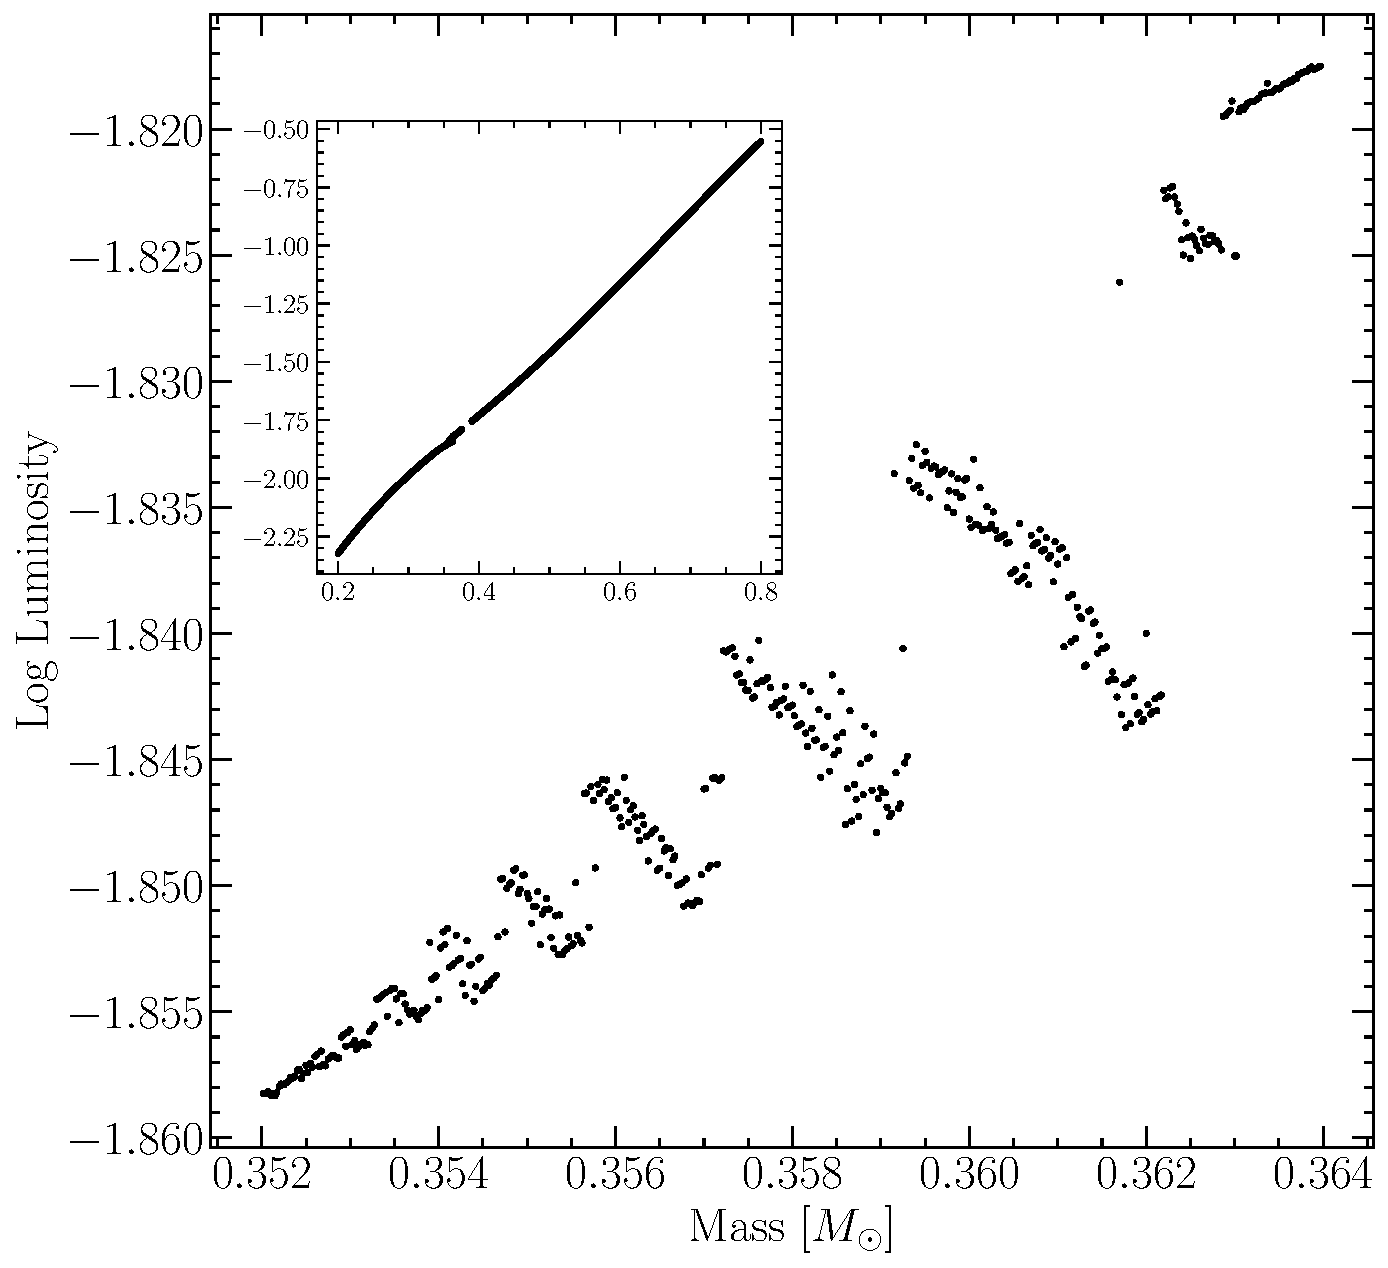
\includegraphics[width=0.45\textwidth]{src/figures/NotebookFigs/OPALPunchIn.pdf}
	\caption{{\color{red} THIS IS A TEST FIGURE, REPLACE WHEN LARGE RUN IS DONE}}
	\label{fig:OPALPunchIn}
	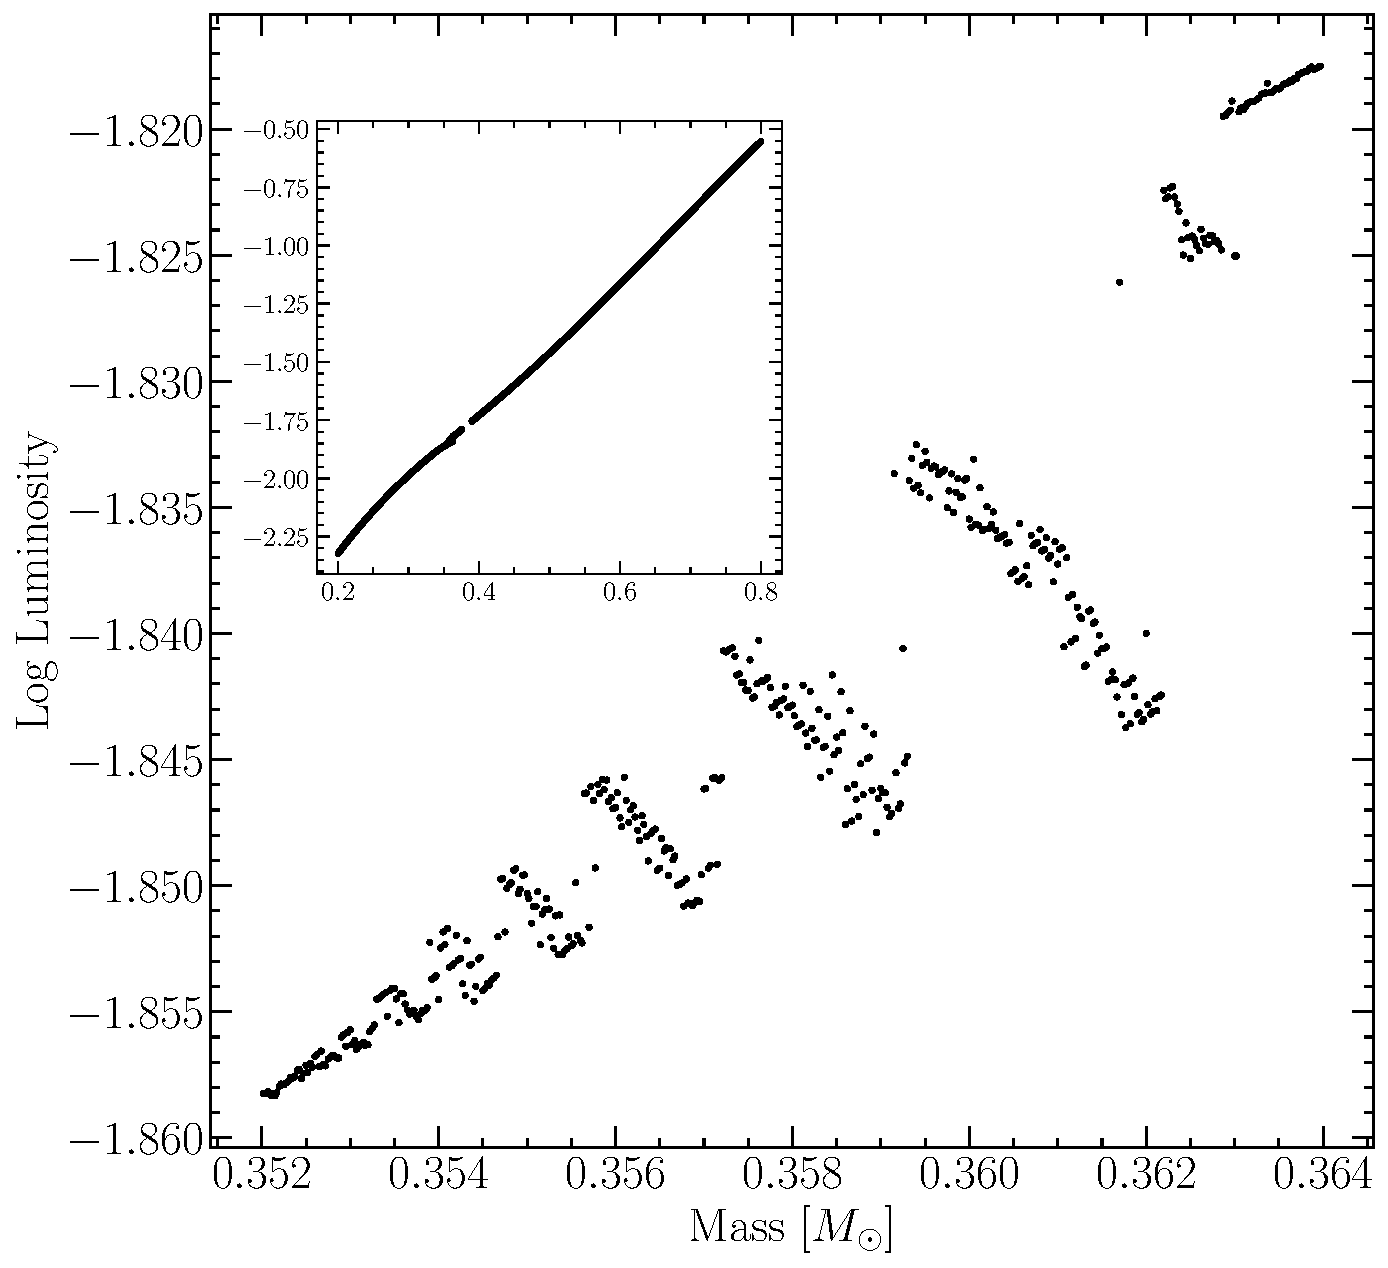
\includegraphics[width=0.45\textwidth]{src/figures/NotebookFigs/OPALPunchIn.pdf}
	\caption{{\color{red} THIS IS A TEST FIGURE, REPLACE WHEN LARGE RUN IS DONE}}
	\label{fig:OPLIBPunchIn}
		
\end{figure}

In order to compare the gap to observations we use in house population
synthetis code {\color{red} describe the population synthetis code then mode
onto the next section, results, include in this a description of how colors are
converted using Aarons code}.


{\color{red} Talk about how you locate the gap formally, there should be a
figure for this as well.}
